%% This template is based on the sample-acmtog template from overleaf.

%% The first command in your LaTeX source must be the \documentclass command.
\documentclass[acmtog, nonacm]{acmart}

%% \BibTeX command to typeset BibTeX logo in the docs
\AtBeginDocument{%
  \providecommand\BibTeX{{%
    \normalfont B\kern-0.5em{\scshape i\kern-0.25em b}\kern-0.8em\TeX}}}

\setcopyright{none}

%%\acmSubmissionID{123-A56-BU3}

%%
%% For managing citations, it is recommended to use bibliography
%% files in BibTeX format.
%%
%% You can then either use BibTeX with the ACM-Reference-Format style,
%% or BibLaTeX with the acmnumeric or acmauthoryear sytles, that include
%% support for advanced citation of software artefact from the
%% biblatex-software package, also separately available on CTAN.
%%
%% Look at the sample-*-biblatex.tex files for templates showcasing
%% the biblatex styles.
%%

%%
%% The majority of ACM publications use numbered citations and
%% references.  The command \citestyle{authoryear} switches to the
%% "author year" style.
%%
%% If you are preparing content for an event
%% sponsored by ACM SIGGRAPH, you must use the "author year" style of
%% citations and references.
\citestyle{acmauthoryear}

%%
%% end of the preamble, start of the body of the document source.
\begin{document}

%% The "title" command has an optional parameter,
%% allowing the author to define a "short title" to be used in page headers.
\title{Simulation of Synthetic Order Book Data with Generative Adversarial Networks}
\subtitle{Scoping document for COMP5530}

%% The "author" command and its associated commands are used to define
%% the authors and their affiliations.
%% Of note is the shared affiliation of the first two authors, and the
%% "authornote" and "authornotemark" commands
%% used to denote shared contribution to the research.
\author{Amazigh Bouldjenet}
\authornote{Sharing first authorship}
\email{sc20amb@leeds.ac.uk}
\author{Chemseddine-Wassim Benimoussa}
\authornotemark[1]
\email{sc20cwb@leeds.ac.uk}
\author{Daniel Lartey}
\authornotemark[1]
\email{sc20dl@leeds.ac.uk}
\author{Panagiotis Magkafas}
\authornotemark[1]
\email{sc20pm@leeds.ac.uk}
\author{Shreyas Honnalli}
\authornotemark[1]
\email{sc20sh@leeds.ac.uk}
\author{Shruti Rajesh Naik}
\authornotemark[1]
\email{sc20srn@leeds.ac.uk}
\author{Sina Ghanbari Saheli}
\authornotemark[1]
\email{sc19sgs@leeds.ac.uk}
\affiliation{%
  \institution{University of Leeds}
  \streetaddress{Woodhouse}
  \city{Leeds}
  \state{West Yorkshire}
  \country{United Kingdom}
  \postcode{LS2 9BW}
}

\author{Dr. Marc de Kamps}
\email{m.dekamps@leeds.ac.uk}
\affiliation{%
  \institution{University of Leeds}
  \country{United Kingdom}}
\additionalaffiliation{the role of Supervisor}

%% By default, the full list of authors will be used in the page
%% headers. Often, this list is too long, and will overlap
%% other information printed in the page headers. This command allows
%% the author to define a more concise list
%% of authors' names for this purpose.
%\renewcommand{\shortauthors}{Dos Anjos, et al.}


%%
%% The code below is generated by the tool at http://dl.acm.org/ccs.cfm.
%% Please copy and paste the code instead of the example below.
%%
\begin{CCSXML}
<ccs2012>
   <concept>
       <concept_id>10010147.10010257.10010321</concept_id>
       <concept_desc>Computing methodologies~Machine learning algorithms</concept_desc>
       <concept_significance>500</concept_significance>
       </concept>
   <concept>
       <concept_id>10010405.10003550</concept_id>
       <concept_desc>Applied computing~Electronic commerce</concept_desc>
       <concept_significance>500</concept_significance>
       </concept>
   <concept>
       <concept_id>10010147.10010341.10010349.10010363</concept_id>
       <concept_desc>Computing methodologies~Data assimilation</concept_desc>
       <concept_significance>500</concept_significance>
       </concept>
 </ccs2012>
\end{CCSXML}

\ccsdesc[500]{Computing methodologies~Machine learning algorithms}
\ccsdesc[500]{Applied computing~Electronic commerce}
\ccsdesc[500]{Computing methodologies~Data assimilation}

%%
%% Keywords. The author(s) should pick words that accurately describe
%% the work being presented. Separate the keywords with commas.
\keywords{GANs, order book, recession, bull market, bear market}

\received{20 February 2007}
\received[revised]{12 March 2009}
\received[accepted]{5 June 2009}

%%
%% This command processes the author and affiliation and title
%% information and builds the first part of the formatted document.
\maketitle

%%
\section{Introduction}
\textcolor{blue}{This section provides an overview for the reader to appreciate the level of challenge posed by the project and its relevance to your degree programme. 
This also demonstrates that you have explored the problem space for the project and have acquired an understanding of the initial requirements.
For a strong start, this section subsections should reflect a systematic and scholarly approach to research or literature review you have undertaken to date.
Don't be afraid to cite relevant papers at this point \cite{graphics}.
Some key things that will most likely be here are:
\begin{itemize}
    \item Context: do not drop the problem and goal out of nowhere. \textbf{Why} is this relevant? Motivation, background drivers, social and/or technical context, stakeholders involved.
    \item Problem statement: a very clear problem statement. It can be a hypothesis, a question that needs to be answered, a statement of the current limitations of existing systems, etc. It can take different forms depending on your project.
    \item Possible solution: Initial thoughts on possible solution(s) to be tackled in the project - what may or may not be pursued depending on speed of progress, challenges and how to approach the development of a potential solution, which modules or computing topics will be the building blocks for the solution.
    Should cite background reading or systematic research conducted so far to provide justification of your initial thoughts.
    \item Validation: If it works, what will you be able to do/prove/see? In essence, how to judge the success of your solution in solving the problem. This will help shaping manageable deliverables. 
\end{itemize}
}

\section{Scope for this project}
\textcolor{black}{The following section specifies the aims, objectives and deliverables of the project. }

\subsection{Aim}
\textcolor{black}{The final product aims to allow users to test trading strategies with realistic data that simulates data in different market conditions.}

\subsection{Objectives}
\textcolor{black}{The key objectives set for the project include.
\begin{itemize}
    \item Build machine learning models that simulate order book data in current market conditions. 
    \item Design a model that uses time series analysis to generate the market data.
    \item Develop an accessible user interface for users to test market strategies. 
\end{itemize}
}

\subsection{Deliverables}
\textcolor{black}{The deliverables for the group project include the following.
\begin{itemize}
    \item Project Report.
    \item Trading Simulation Software.
    \item Video Demonstration of the Software.
    \item GitHub Code Repository. 
\end{itemize}
}

\section{Project schedule}
\textcolor{blue}{Talk shortly about how you came up with the plan that you are about to present. The schedule for completion of the project should relate the activities (or tasks) to objectives or deliverables. A few milestones should be identified for self monitoring of progress.
}

\subsection{Methodology}
\textcolor{blue}{Outline the underpinning project approach that is appropriate for the chosen type of project. This should help to plan for the order of the activities/tasks}


\subsection{Tasks, milestones and timeline}
\textcolor{black}{The project consists of three fundamental phases: (1) planning and research, (2) implementation and testing, and (3) report writing. Figure 1 illustrates the expected timeline for product development. 
\begin{figure}[htp]
    \centering
    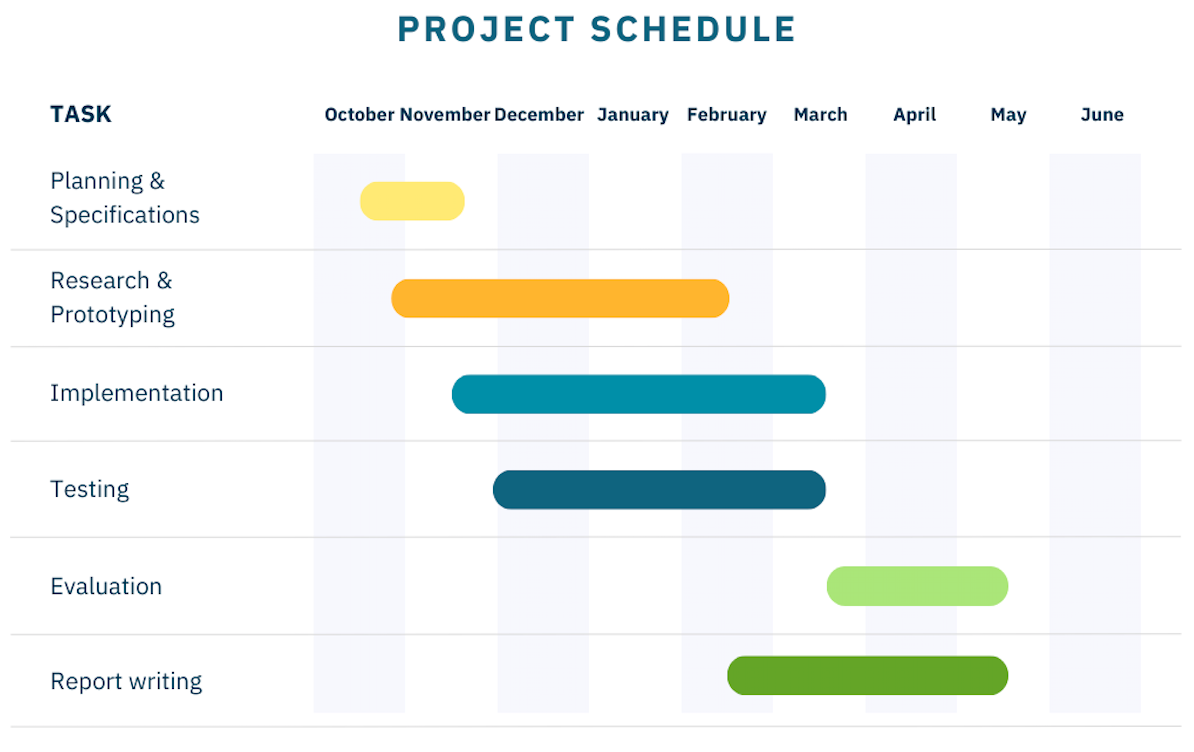
\includegraphics[width=8cm]{project-timeline.png}
    \caption{Timeline of Project Schedule}
    \label{fig:schedule}
\end{figure}}

\textcolor{black}{The initial phase involves developing prototype solutions and devising a project specification with the final aims and objectives. During the implementation phase, the group will utilise both unit and integration testing to ensure code quality. Finally, the group aims to have a completed product by March to conduct an evaluation of the software using user reviews and automated performance tests. }

\subsection{Risk assessment}
\textcolor{red}{Prior to the development process, the group conducted a risk assessment to explore the various strengths and constraints of the project. 
\newline\newline --- Still working on it, feel free to add --- }
\textcolor{black}{
\begin{table}[h]
  \centering
  \begin{tabular}{| {0.1\linewidth} | p{0.3\linewidth} | p{0.4\linewidth} |}
    \toprule
    No. & Risk or Issue & Strategies to resolve \\
    \midrule
        1 & Project Viability & Conduct a Project Viability Assessment to explore technical concerns. \\
        2 & Project Completion & Use of weekly sprints and scrum methods.\\
        3 & Data Abundance and Quality & Merging datasets from various sources and thorough data quality inspection. \\
        4 & Implementing new technologies & Weekly group meetings to discuss any concerns and struggles. \\
        5 & Model Over-fitting & Use of techniques such as data pruning, cross-validation and regularization. \\
        6 & Evaluation Process & Conduct in-person user trials to discover potential user experience or technical constraints. \\
    \bottomrule
  \end{tabular}
  \caption{Summary of Potential Project Risks}
\end{table}
}
%%
%% The next two lines define the bibliography style to be used, and
%% the bibliography file.
\bibliographystyle{ACM-Reference-Format}
\begin{thebibliography}{9}
Alibašić, H., 2023. Developing an Ethical Framework for Responsible Artificial Intelligence (AI) and Machine Learning (ML) Applications in Cryptocurrency Trading: A Consequentialism Ethics Analysis. \textit{FinTech}, \textbf{2}(3), pp.430-443. \textit{Available from:} https://www.mdpi.com/2674-1032/2/3/24 \newline 
Coinbase., 2023. Coinbase pricing and fees disclosures. [online] \textit{Available from:} https://help.coinbase.com/en/coinbase/trading-and-funding/pricing-and-fees/fees.\newline
Coinbase., 2023. Code of Business Conduct and Ethics Global.[online] \textit{Available from: }https://s27.q4cdn.com/397450999/files/doc\_downloads/gov\_docs/Code-of-Business-Conduct-Ethics-Global-(252092)-Coinbase.com-Web-(1).pdf \newline
Olcay Sonkurt, H., 2023. Cryptocurrency Trading as a Behavioral Addiction: A Case Report. \textit{Psychiatria Danubina}, \textbf{35}(1), pp.128-131. [online] \textit{Available from:} https://hrcak.srce.hr/file/443600 \newline
\end{thebibliography}


\appendix

\section{How ethical issues are addressed}
\setlength{\parindent}{20pt}
\textcolor{black}{The project scope involves the use of machine learning in the finance and trading industry, which has numerous ethical concerns. Alibašić (2023) presents how the use of machine learning in trading is likely to produce biased or misleading results due to market volatility. Further, the author highlights how using publicly available data suggests that trading privacy is primarily non-existent, and traders must be made aware of this transparency (Alibašić, 2023).}

\textcolor{black}{To help mitigate this issue, Alibašić (2023) suggests a three-part evaluation framework to assess the morality of the designed software: (1) Developed algorithms should emphasise responsible trading (2) Software should cause minimal harm to users (3) Developed software should be transparent and held accountable for miscalculations. The group aims to periodically revisit these traits throughout the project to assess and ensure the final product upholds these ethical standards.}

\textcolor{black}{Another critical concern with the final software is its impact on users. Trading addiction, specifically with cryptocurrency, has been studied as a subclass of gambling addiction (Olcay Sonkurt, H., 2023). The case study emphasises how the disorder is most common in those with previous addictions and occurs due to the risk appeal of market instability (Olcay Sonkurt, H., 2023). Unsupervised and miscalculated trading may result in extreme measures taken by users. For instance, if the software predicts a false outcome to a user's tested strategy and encourages the user to make a trading decision resulting in financial loss, it could emotionally distress the user and provoke them to make extreme decisions. This scenario would not only be a liability for the software but also be an ethical concern. Although the software seeks to simulate the actual marketplace, it must provide disclaimers to users regarding the possibility of misleading predictions to help mitigate this moral issue.}

\textcolor{black}{Finally, the project utilises public cryptocurrency data supplied by a Coinbase API to build and maintain a real-time Order Book. Coinbase is an online platform facilitating secure cryptocurrency trading by charging a small fee per trade transaction (Coinbase., 2023). Before implementing this API, the group examined the ethical standing of the firm. According to the Code of Conduct, the firm is in compliance with all international governmental regulations and seeks to be an ethical business. (Coinbase., 2023). 
}
\end{document}
\endinput
%%
%% End of file `scoping-document.tex'.
